% This example An LaTeX document showing how to use the l3proj class to
% write your report. Use pdflatex and bibtex to process the file, creating 
% a PDF file as output (there is no need to use dvips when using pdflatex).
% Modified 

% This dissertation was built upon base template provided.

\documentclass{l3proj}

\begin{document}

\title{Team I: ResDiary Restaurant Recommendation System}

\author{Vladimir Bardarski \\
        Paulius Dilkas \\
        Domantas Jurkus \\
        Edward Kalfov \\
        Josh O'brien \\
		Joseph O'Hagan}

\date{31st March 2017}

\maketitle

% ##################################################
% LAST EDIT: 	06/03/17	Joseph
% ##################################################
\begin{abstract}
The abstract shall go here! Here is some things to keep in mind while writing it.
\end{abstract}

\begin{itemize}
\item The abstract is likely the first substantive description of your work read by an examiner. View it as an opportunity to set accurate expectations.
\item The abstract is a summary of the whole thesis. It presents all the major elements of your work in a highly condensed form. (Write it having written the rest of the paper) The paper sets the abstract.
\item It must be capable of substituting for the whole paper when there is insufficient time and space for the full text.
\item Keep it short and snappy. 
\item The primary function of your thesis (and by extension your abstract) is not to tell readers what you did, it is to tell them what you discovered.
\item Approximately the last half of the abstract should be dedicated to summarizing and interpreting your results.
\item The most common error in abstracts is failure to present results.
\end{itemize}

% Comment out this line if you do not wish to give consent for your work to be distributed in electronic format.
% We hereby give consent - spread the knowledge - pending on result of project
\educationalconsent
s
\newpage

%==============================================================================

% ##################################################
% LAST EDIT: 	06/03/17	Josh
% ##################################################
\section{Introduction}
% An introduction, explaining the purpose of the document, a very brief outline of the project and a summary of the structure of the rest of the document (approximately 1-2 pages).

The Professional Software Development (PSD3) course at The University of Glasgow requires students to engage with the practices and methodologies used in modern large-scale software engineering. The purpose of this dissertation is to document the development of the software project created as part of this course by Team I. 

The project was to build, over the course of several months, a restaurant recommendation engine for the Glasgow-based company ResDiary.
The goal was to deliver a system which could produce recommendations for restaurants to a user, that could be integrated into their existing systems at a later date. 
% Do we delay mentioning the integration at this stage? - Joseph?
% Do we make it clear here it was recommendations based on similar users? - Joseph?

Our team consisted of six third-year Computing Science students. Within the group there was a broad array of skills, interests and experience - with two members actively working as software professionals, and another having participated in an internship. For some members, however, this was a first opportunity to interact with a real client. 

In this document we outline, in detail, the entire process: from the initial requirements gathering with our customer, through to final system delivery. 

In section \ref{sec:background} we present the background to the project, the motivations of the customer and how we arrived at the agreed deliverables.

%this will surely be expanded to enumerate each separate section better I would like to discuss in detail the practices, issue-tracking, the team work/team load - Josh etc.

In subsequent sections \ref{sec:alice} through Section \ref{sec:reflections} we explore the challenges we faced through development and the steps we took to resolve them, explore the impact of team dynamics on the outcome and reflect on what we have learned from the experience. We also explain how we applied the good development practices learned in PSD3. In particular we highlight the role of version control, agile development and issue tracking.

\newpage

%==============================================================================

\section{Case Study Background}
\label{sec:background}
% A description of the case study background and context. This should include a description of the project customer (what was the nature of the organisation you were working for), their objectives for the project, and a summary of what was actually achieved. Where appropriate, this section should also make reference to similar related projects in order to make the context clear (approximately 4-5 pages).

% MISC POINTS TO DISCUSS:
% 1. Do we address the legal contract we signed. I.e. Initially it was proposed for integration into the site. It then changed and this we reflected in the contract we signed which outlined the final product and how it could be used be ResDiary - possibly get a more accurate summary of what ResDiary can do with the delivered product from them (ask them to summarise the contract essentially mentioning it is beneficial to our final report)

% ##################################################
% LAST EDIT: 	12/03/17	Joseph
% ##################################################
\subsection{Customer}
\label{customer}
% The customer organisation and background.

% Here we want answer the question of who are ResDiary and what do they do.
% Additionally answer who played the customer role of ResDiary to us on the project.

% Who are ResDiary?
ResDiary are a Glasgow-based online restaurant reservation system. They are a commercial organisation whose service provides a comprehensive, easy to use booking platform and table management system for use by both the hospitality industry and its guests. The service provides 24-hour reservation services via websites including Facebook and Twitter as well as their own booking portal ResDiary.com. Their global service sees 9.7 million covers booked every month and their technology is in use in over 6,500 restaurants across 58 countries.

Throughout the duration of the project ResDiary senior software engineers Adam Connelly and Ian Strachan acted as the representatives of ResDairy. They served as the point of contact between our team and the customer and provided useful feedback and answers to our queries throughout the development of the project. Additionally they also provided supplies of data for use within the project with the necessary steps taken by ResDiary to ensure the anonymity of their sensitive customer data.

% ##################################################
% LAST EDIT: 	12/03/17	Joseph
% ##################################################
\subsection{Customer Objectives And Rationale}
\label{custobjectives}
% The rationale and initial objectives for the project.

% Essentially with the intro we want to introduce the company and the aims of the project. Mention similar real world examples such as the Netflix model as this was used as a reference / example similar project early on in our project. Talk out the specification, reference the dropped features of the specification in relation to what was actually developed and presented to the customer. Potentially mention points of future expansion as well and how project was setup to account for those future developments.

% Possibly reflect on the change in specification that occurred - how it was originally proposed to what it evenually became both from our perspective (in terms of what we would develop) and how ResDiary wished to use the project (in that they intially proposed either integrating it into their system or creating an API to eventually just wanting it as a proof of concept to learn from).

% Essentially I want to introduce the customer and provide an overview of the motivation of the project.
% Project motivation comes from three reasons:
% 1. Improve restaurant discover on existing service 
%	2. Commerial reason as it is not something their competition does
%	3. Big data proof of concept research - they have large amount of big data they do nothing with and would like to see if using it for such a purpose would be useful

% This is rough but I'm trying to mainly hit on the motives and tease on some later developments


% Initial Meeting - Project Motivation - Initial Aims

The initial customer meeting occurred on October 19th and was led by Ian Strachan. This was our first contact with the customer and served as the customer requirements elicitation meeting. The meeting began with an overview of the ResDairy business (link to customer section above) and some background was given of the technologies of their system currently in place. This included some information on the particular development languages being used (primarily C\#) though the primary justification was to provide background context for the large quantities of data being gathered by ResDiary from their day-to-day operations. This large mass of big data however is currently unused and dormant which ResDiary view as a significant shortcoming of their existing system. 

Through utilisation of this large quantity of data they believe they will be able to distinguish themselves and gain a commercial edge over their competition. Having conducted some research they have found that none of their competitors currently offer a restaurant recommendation service within their particular booking platform. They believe such as system which makes recommendations to users based off their previous dining habits and similarity to other users will give them the edge over their competition. Additionally their belief is that such a feature will increase restaurant discovery on their service which will be of benefit to both their customers and the organisation itself.

The idea stems from the similar system provided by services such as Amazon and Netflix. The Netflix model in particular being the closest reference point for the system they wished to replicate due the intrinsic similarity between making recommendations based on a user’s history and similarity to other users tastes. As a starting point for our own research to understand attempts to solve similar problems they suggested looking into the 2009 Netflix Prize competition. The goal competition was to produce the best algorithm which could accurately predict a user’s rating of a film based on previous ratings and no other additional information about the users or the films.

While the primary focus of the project was to develop the recommendation system as a proof of concept for ResDiary, some time was spent discussing the potential of integrating the system into the existing ResDiary system. The proposed method was through the creation an API to link the two systems together though the customer elucidated our primary focus should be create the recommendation engine as this final goal was susceptible to change. This in part they explained was due to an internal transition in development technologies for the back end functionality of their service. As such whether the project would be integrated into the existing service or alternatively viewed as an R\&D project for a potential use of their big data had not yet been decided by the customer. 

Ultimately it would be the latter of the two as the customer wished to view the project as a proof of concept to assess the benefits of utilising their big data in such a manner. Whether the additional development costs associated with integration would outweigh the benefits provided and whether the system could make smart recommendations based off the existing data provided to it. Through examining our system they believed they could answer such questions and use our system as a starting point to learn from so that a similar system could be integrating into their existing service.


\subsection{Our Initial Objectives And Rationale}
\label{ourinitobjectives}
% ##################################################
% LAST EDIT:  14/03/17  Joseph
% NOTE:         Requires subsectioning
% NOTE:         Needs reworking
% NOTE:			Needs referencing
% NOTE:			Needs cutting down page count 
% ##################################################

% Present our initial takeaways and how we came to them
% Tease some of the various changes which occurred along the way
% Lead into the final state of the system 

% Here is our interpretation of their requirements pitched above
% Here are their adjustments based off our initial interpretation of their requirements

% Reference the Netflix / additional research / similar systems here

% There are 4 main stages - initial assumptions - refinements after first meeting - refinements after January meeting - final state of the project.


Having conducted the requirements elicitation meeting the team dedicated the next few weeks to performing the necessary background research associated with the project. This occurred in tandem with the production of a formal requirements specification which would serve as the project proposal document presented to the client at the next customer meeting on November 16th. This document contained the proposed functional and nonfunctional requirements the team decided upon for the project and a set of user stories (ranked by priority) which were then subdivided into individual tasks. In addition a proposed high-level system UML diagram was included and a step-by-step workflow of how the system would generate recommendations was presented. 

The team agreed upon the functional and nonfunctional requirements of the project based upon our interpretation of the customer’s pitch at the requirements elicitation meeting. Although these would later be revised and refined as the project developed it was initially proposed for the project to meet the following functional and nonfunctional requirements:

Initial functional requirements (!!! subsection !!!):
\begin{itemize}
\item The recommendation engine must accurately suggest restaurants based on the user’s dining history and similarity to other users with similar eating preferences.
\item Recommended restaurants should be in close proximity to where the user typically eats or the geographical location of where they are currently searching.
\item The recommendation engine may recommend restaurants the user has previously visited should the user optionally select for this to occur.
\end{itemize}

Initial nonfunctional requirements (!!! subsection !!!):
\begin{itemize}
\item The engine should be written to allow for easy integration into the existing Resdiary system.
\item The system should give a response within 1 second after receiving the request (provided data is stored locally).
\item New users should be presented an optional quick questionnaire to gather initial data.
\item User and restaurant locations should be interpreted using coordinates rather than city  name as those are of arbitrary precision within the dataset.
\end{itemize}

As the customer’s vision of the final state of the project was suspect to change, the proposed final state of the project was left it intentionally vague and the specification written to allow for flexibility on the customer’s part. Instead the focus was placed on building and producing the most accurate recommendation for a given user. As both the team and customer felt this to be the most critical aspect of the system a significant portion of time was devoted at the outset of the project to ensuring the proposed system was in fact the correct system to be built.  

The higher level system diagram was based upon... 

Upon presentation to the customer, the customer felt we had a good understanding of their desire for the system. They agreed with our proposed functional requirements and envisioned how the high level system would operate in relation to their existing system. The customer did express concern however regarding the proposed response rate of the system and felt the need to further clarify the volume of data the system would be expected to work with. To combat this a nightly build system was suggested as this is what they anticipated should they wish to implement the system. Regarding our proposed high level system they particularly expressed interest in being able to “fine tune” the system through altering the significance place on individual recommenders. Finally the customer suggested developing a lightweight front end application to display the recommendations. They conceded that such a development feature was throwaway as their interest was in the recommendation system itself but rationalised its development with the belief that such an application would help them to better understand the system, to assist demonstrate the functionality of the system visually and give a clear indication of if the system was producing sensible results. 

Responding to this feedback the team felt the need to revise the nonfunctional requirements of the project. This saw the removal of the aforementioned “1 second local response 
rate” and the introduction of the following two new requirements:

\begin{itemize}
\item Provided the data is not stored locally, the system should be setup to allow for nightly updates to the recommendations made.
\item Have the ability to “fine tune” the recommendation engine by altering the weighting significance of different components of the recommendation such as distance, price, 
reviews, etc.
\end{itemize}

In addition the team also introduced the aim of producing a lightweight front end display to showcase the recommendation system. We agreed with the customers belief that this would help showcase the system and provide a visual method for non-technical users to see the results of our work. As the customer was still unclear of the final form of the system, proof of concept or actual integration, both parties decided to delay the decision until the scheduled meeting on January 26th. This would allow for significant development time on the application to occur and would grant the customer more time to determine their use for the system in relation to their business needs at that time. 

Upon presenting the progress made at the January 26th meeting the team pressed the customer regarding what their vision for the final state of the system would be. Having discussed this issue with the customer it became clear they wished to view the project as “proof-of-concept” system. That their intended use of the system was to assess the worth of creating a similar system for their existing system. Additionally they wished to learn from the system as they have little experience in this particular field. Finally should they believe a similar system to be of use to their business, they wished to use our system as a prototype to justify the resources required for development of a similar system to the non-technical members of their company.

With the final handover state of the system known, the team decided a redesign of the front end of the application was necessary. . The primary justification for this redesign came through an observation made while giving the demonstration at the January 26th meeting. As ResDiary software engineer Adam Connelly was unable to attend the meeting due to other commitments, a non-technical member of the ResDiary team joined Ian Strachan during the meeting. From this non-technical perspective it was clear to the team that the system was not properly communicating the recommendations being made. It was unclear to a non-technical user how the system generally operated, if it was functioning correctly and if the results it produced looked sensible. The aim of this redesign then was to visually show the system was operating correctly and producing accurate predictions. With a clearly defined end state for the system the following functional requirements were discovered and added to the project:

Functional
\begin{itemize}
\item The front end display should display recommendations for a random pool of users to simulate typical use of the system.
\end{itemize}

Nonfunctional
\begin{itemize}
\item The front end be designed such that it is aesthetically clear that the recommendations made are sensible and accurate.
\end{itemize}

With this defined endpoint... the development continued on until the end of the project.

Although development continued at a steady pace between the January 26th meeting and the final meeting scheduled for March 22nd the decision was in the aftermath of the January meeting to drop the proposed nonfunctional requirement of creating a quiz to make recommendations for new users. While this particular feature was viewed as a bonus feature the team felt based on the customer’s feedback that they were not particularly interested in this feature. The earlier conducted research showed that making recommendations of this type was primarily a search based recommendation whereas the customer’s interests lay in recommendations made through user similarity. As such the development resources were instead focused on the aforementioned goals of producing a more accurate collaborative and content based recommendation system and the production of a high quality front end to professionally display system output. 

% ##################################################
% LAST EDIT: 	06/03/17	Joseph
% ##################################################
\subsection{Delivered Software}
\label{finsoftware}
% Information on the final software that was delivered to the customer.

\newpage

%==============================================================================
\section{Alice}
\label{sec:alice}

This is a example of how to include an image from the figures directory.

\begin{figure}
\begin{center}
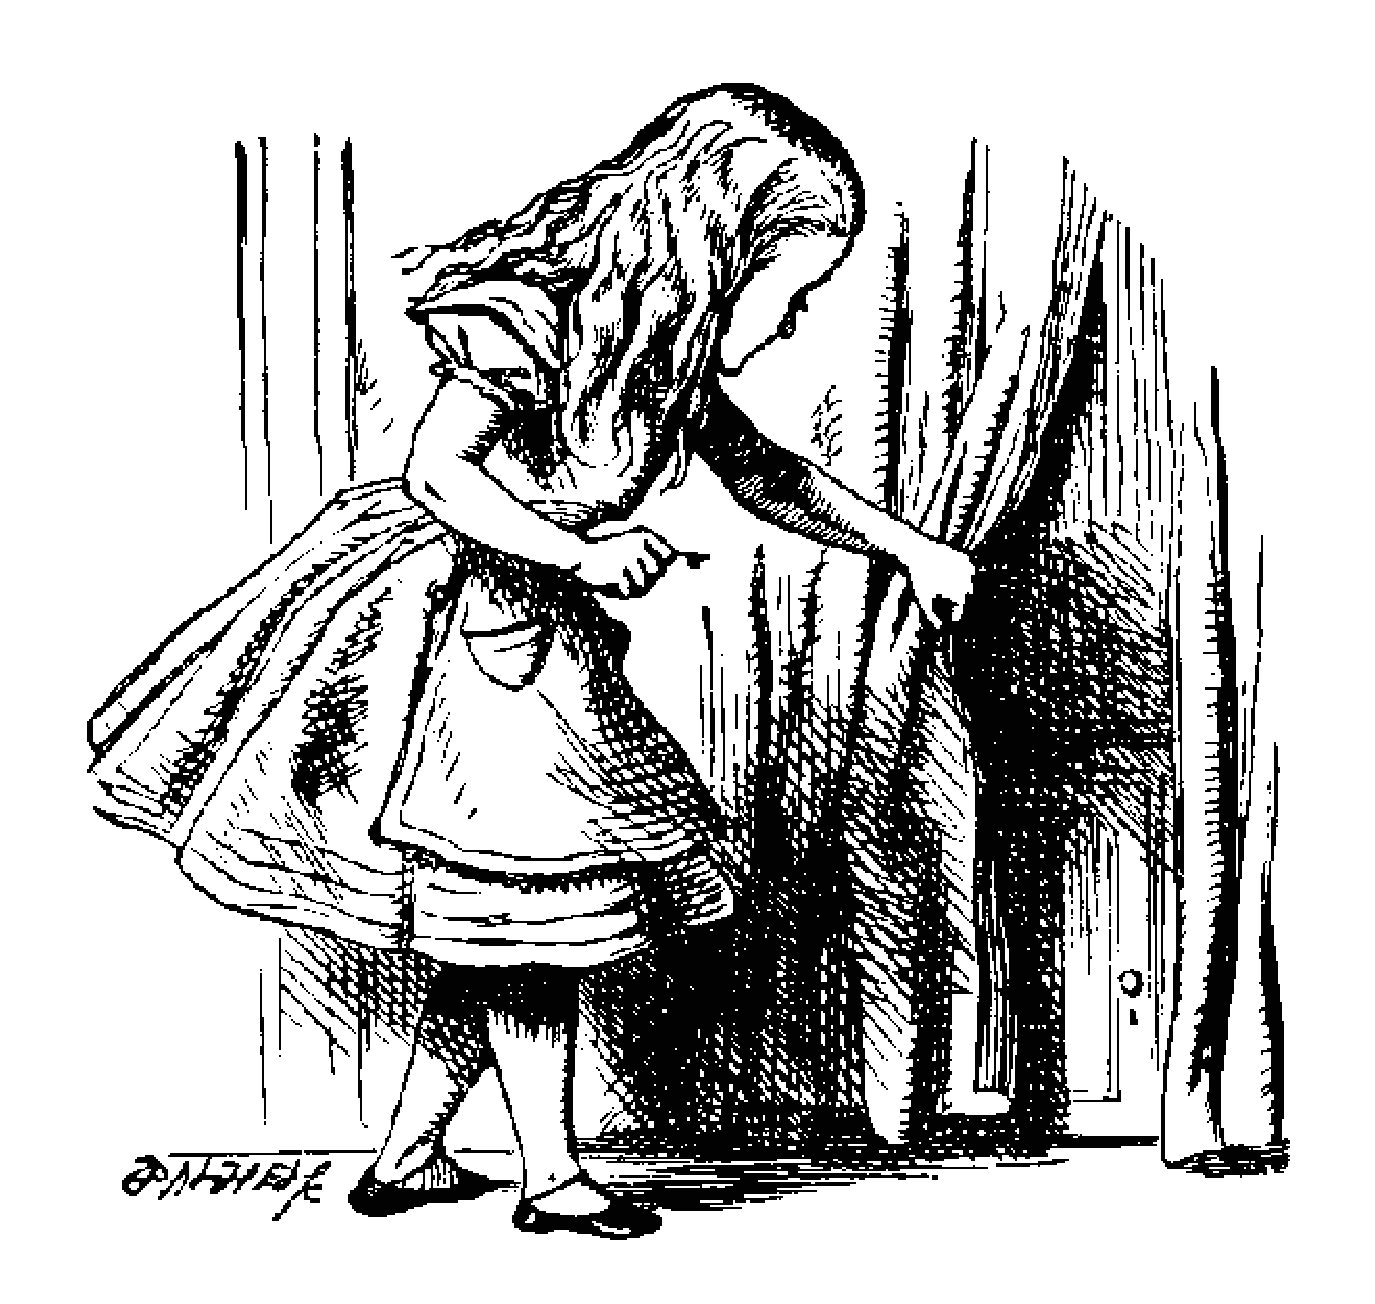
\includegraphics[width=7cm]{figures/alice}
\end{center}
\caption{Behind it was a little door}
\label{fig:alice}
\end{figure}

This is an example of how to reference an inlcuded figure (see Figure \ref{fig:alice}).

%==============================================================================
\section{Reflections}
\label{sec:reflections}

% Several sections that reflect on your experiences during the team project. Each section should discuss one theme, characterised by incidents or events that occurred during the team course of the project from which you learned (approximately 12-15 pages).

%==============================================================================
\section{Conclusions}
\label{sec:conclusions}
% A conclusion that draws general and wider lessons from the case study (approximately 1-2 pages)

Explain the wider lessons that you learned about software engineering,
based on the specific issues discussed in previous sections.  Reflect
on the extent to which these lessons could be generalised to other
types of software project.  Relate the wider lessons to others
reported in case studies in the software engineering literature.

%==============================================================================
\bibliographystyle{plain}
\bibliography{dissertation}
\end{document}
